% !TeX vek = sv_SE
%http://www.cs.put.poznan.pl/ksiek/latexmath.html
%https://en.wikibooks.org/wiki/LaTeX/Advanced_Mathematics
%http://www.maths.lth.se/matematiklth/personal/magnusa/kurser/endim-ht2015/B1/kurspmB1ht15.pdf

\documentclass[a4paper]{article} 
\usepackage[T1]{fontenc} 
\usepackage[utf8]{inputenc} 
\usepackage[swedish]{babel} 
\usepackage{amsmath}
\usepackage{amssymb}
\usepackage{cancel}
\usepackage{graphicx}
\usepackage{systeme}

\setlength\arraycolsep{0pt}

\usepackage{color}
\definecolor{tskcol}{RGB}{193,70,70}
\newcommand{\tskcol}[1]{\textcolor{tskcol}{#1}}

\newcommand{\vek}[1]{\overrightarrow{#1}}

\newcommand\varpm{\mathbin{\vcenter{\hbox{%
				\oalign{\hfil$\scriptstyle+$\hfil\cr
					\noalign{\kern-.5ex}					
					$\scriptscriptstyle({-})$\cr}%
			}}}}
			
			\setlength{\parindent}{0in}
			

\title{Linjär algebra\\ FMA420} 
\author{Emil Wihlander\\ dat15ewi@student.lu.se} 
\date{2016--05--12}
\begin{document} 
\maketitle
\pagebreak
\section*{Kapitel 1: Linjära ekvationssystem}
\texttt{\tskcol{1.1~~~~~ (s.)}}
\begin{quotation}
	\noindent
	Börja nerifrån och upp och lös en variabel i taget.
	\begin{align*}
	&\systeme{
		2x+3y- z=5,
		  -3y+5z=1,
		      4z=8}  \\ \Leftrightarrow
	&\begin{cases}
	z=2 \\
	y=\frac{1-5*2}{-3}=3 \\
	x=\frac{5+2-3*3}{2}=-1
	\end{cases}
	\end{align*}
	\\
	\textbf{Svar:} $(x,y,z)=(-1,3,2)$
\end{quotation}

\texttt{\tskcol{1.2~~~~~ (s.)}}
\begin{quotation}
	\noindent
	Gausselimination:
	\begin{align*}
	&\systeme{
		  x-2y+  z=2,
		 2x-6y+11z=35,
		-3x+5y+  z=8}  
	&\begin{array}{l} 
		(a) \\ 
		(b) \\
		(c)
	\end{array} \\ \Leftrightarrow
	&\systeme{
		x-2y+ z=2,
		 -2y+9z=31,
		 - y+4z=14}  
	&\begin{array}{l} 
	(a')=(a) \\ 
	(b')=(b)-2(a) \\
	(c')=(c)+3(a)
	\end{array} \\ \Leftrightarrow
	&\systeme{
		x-2y+   z=2,
		 -2y+  9z=31,
		    -\frac{1}{2}z=-\frac{3}{2}}  
	&\begin{array}{l} 
	(a'')=(a') \\ 
	(b'')=(b') \\
	(c'')=(c')-\frac{1}{2}(b')
	\end{array} \\ \Leftrightarrow
	&\begin{cases}
	z=3 \\
	y=\frac{31-9*3}{-2} =-2\\
	x=2+2*(-2)-3=-5
	\end{cases}
	\end{align*}
	\\
	\textbf{Svar:} $(x,y,z)=(-5,-2,3)$
\end{quotation}

\pagebreak
\texttt{\tskcol{1.3~~~~~ (s.)}}
\begin{quotation}
	\noindent
	Gausselimination:
	\begin{align*}
		&\systeme{
			  x-2y+ z=1,
			 2x-6y+6z=2,
			-3x+5y+ z=3}  
		&\begin{array}{l} 
			(a) \\ 
			(b) \\
			(c)
		\end{array} \\ \Leftrightarrow
		&\systeme{
			x-2y+ z=1,
			 -2y+4z=0,
			 - y+4z=6}  
		&\begin{array}{l} 
			(a')=(a) \\ 
			(b')=(b)-2(a) \\
			(c')=(c)+3(a)
		\end{array} \\ \Leftrightarrow
		&\systeme{
			x-2y+ z=1,
			 -2y+4z=0,
			     2z=6}  
		&\begin{array}{l} 
			(a'')=(a') \\ 
			(b'')=(b') \\
			(c'')=(c')-\frac{1}{2}(b')
		\end{array} \\ \Leftrightarrow
		&\begin{cases}
			z=3 \\
			y=\frac{-4*3}{-2} =6\\
			x=1+2*6-3=10
		\end{cases}
	\end{align*}
	\\
	\textbf{Svar:} $(x,y,z)=(10,6,3)$
\end{quotation}

\texttt{\tskcol{1.4~~~~~ (s.)}}
\begin{quotation}
	\noindent
	Gausselimination:
	\begin{align*}
	&\systeme{
		  x-2y+ z=1,
		 2x-6y+6z=2,
		-3x+5y- z=3}  
	&\begin{array}{l} 
	(a) \\ 
	(b) \\
	(c)
	\end{array} \\ \Leftrightarrow
	&\systeme{
		x-2y+ z=1,
		 -2y+4z=0,
		 - y+2z=6}  
	&\begin{array}{l} 
	(a')=(a) \\ 
	(b')=(b)-2(a) \\
	(c')=(c)+3(a)
	\end{array} \\ \Leftrightarrow
	&\systeme{
		x-2y+ z=1,
		 -2y+4z=0,
		      0z=6}  
	&\begin{array}{l} 
	(a'')=(a') \\ 
	(b'')=(b') \\
	(c'')=(c')-\frac{1}{2}(b')
	\end{array}
	\end{align*}
	Saknar lösning eftersom $0\neq6$.
	\\ \\
	\textbf{Svar:} Lösning saknas
\end{quotation}

\pagebreak
\texttt{\tskcol{1.5~~~~~ (s.)}}
\begin{quotation}
	\noindent
	Gausselimination:
	\begin{align*}
		&\systeme{
			 2x-6y+11z=35,
			  x-2y+  z=2,
			-3x+5y+  z=8}  
		&\begin{array}{l} 
		(a) \\ 
		(b) \\
		(c)
		\end{array} \\ \Leftrightarrow
		&\systeme{
			x-2y+  z=2,
			2x-6y+11z=35,
			-3x+5y+  z=8}  
		&\begin{array}{l} 
		(a')=(b) \\ 
		(b')=(a) \\
		(c')=(c)
		\end{array}
	\end{align*}
	Lös som i \texttt{\tskcol{1.2}}
	\\ \\
	\textbf{Svar:} $(x,y,z)=(-5,-2,3)$
\end{quotation}

\texttt{\tskcol{1.6~~~~~ (s.)}}
\begin{quotation}
	\noindent
	Gausselimination:
	\begin{align*}
	&\systeme{
		  x-2y+3z=1,
		 2x-4y+7z=3,
		-3x+5y- z=2}  
	&\begin{array}{l} 
	(a) \\ 
	(b) \\
	(c)
	\end{array} \\ \Leftrightarrow
	&\systeme{
		  x-2y+3z=1,
		        z=1,
		   - y+8z=5}  
	&\begin{array}{l} 
	(a')=(a) \\ 
	(b')=(b)-2(a) \\
	(c')=(c)+3(a)
	\end{array} \\ \Leftrightarrow
	&\systeme{
		x-2y+3z=1,
		 - y+8z=5,
		      z=1}  
	&\begin{array}{l} 
	(a'')=(a') \\ 
	(b'')=(c') \\
	(c'')=(b')
	\end{array} \\ \Leftrightarrow
	&\begin{cases}
	z=1 \\
	y=-(5-8*1)=3\\
	x=1+2*3-3*1=4
	\end{cases}
	\end{align*}
	\\
	\textbf{Svar:} $(x,y,z)=(4,3,1)$
\end{quotation}

\pagebreak
\texttt{\tskcol{1.7~~~~~ (s.)}}
\begin{quotation}
	\noindent
	Gausselimination:
	\begin{align*}
		&\systeme{
			  x- y-2z+ 2w=-1,
			-3x+4y+7z-12w=2,
			 2x-4y-3z- 2w=-12,
			 5x- y-3z-31w=-20}  
		&\begin{array}{l} 
		(a) \\ 
		(b) \\
		(c) \\
		(d)
		\end{array} \\ \Leftrightarrow
		&\systeme{
			x- y-2z+ 2w=-1,
			   y+ z- 6w=-1,
			 -2y+ z- 6w=-10,
			  4y+7z-41w=-15}  
		&\begin{array}{l} 
		(a')=(a) \\ 
		(b')=(b)+3(a) \\
		(c')=(c)-2(a) \\
		(d')=(d)-5(a)
		\end{array} \\ \Leftrightarrow
		&\systeme{
			x- y-2z+ 2w=-1,
			   y+ z- 6w=-1,
			     3z-18w=-12,
			     3z-17w=-11}  
		&\begin{array}{l} 
		(a'')=(a') \\ 
		(b'')=(b') \\
		(c'')=(c')+2(b') \\
		(d'')=(d')-4(b')
		\end{array} \\ \Leftrightarrow
		&\systeme{
			x- y-2z+ 2w=-1,
			   y+ z- 6w=-1,
			     3z-18w=-12,
			          w=1}  
		&\begin{array}{l} 
		(a''')=(a'') \\ 
		(b''')=(b'') \\
		(c''')=(c'') \\
		(d''')=(d'')-(c'')
		\end{array} \\ \Leftrightarrow
		&\begin{cases}
		w=1 \\
		z=\frac{-12+18*1}{3}=2 \\
		y=-1-2+6*1=3\\
		x=-1+3+2*2-2*1=4
		\end{cases}
	\end{align*}
	\\
	\textbf{Svar:} $(x,y,z,w)=(4,3,2,1)$
\end{quotation}

\texttt{\tskcol{1.8~~~~~ (s.)}}
\begin{quotation}
	\noindent
	Eftersom det endast är två variabler krävs endast två ekvationer för att lösa systemet. Testa sedan mot resterande ekvationer för att se om systemet har en lösning.
	
	Gausselimination:
	\begin{align*}
		&\systeme{
			  x-2y=1,
			 3x+4y=13,
			-5x+2y=-13,
			 4x-3y=9}  
		&\begin{array}{l} 
		(a) \\ 
		(b) \\
		(c) \\
		(d)
		\end{array} \\ \Leftrightarrow
		&\systeme{
			  x- 2y=1,
			    10y=10}  
		&\begin{array}{l} 
		(a')=(a) \\ 
		(b')=(b)-3(a)
		\end{array} \\ \Leftrightarrow
		&\begin{cases}
		y=1 \\
		x=1+2*1=3
		\end{cases}
	\end{align*}
	Kolla $(c)$ och $(d)$:
	\[-5*3+2*1=-13\]
	\[4*3-3*1=9\]
	\\
	\textbf{Svar:} $(x,y)=(3,1)$
\end{quotation}

\texttt{\tskcol{1.9~~~~~ (s.)}}
\begin{quotation}
	\noindent
	Eftersom det endast är två variabler krävs endast två ekvationer för att lösa systemet. Testa sedan mot sista ekvationen för att se om systemet har en lösning.
	
	Gausselimination:
	\begin{align*}
	&\systeme{
		 x+ y=-4,
		 x-2y=2,
		3x+4y=1}  
	&\begin{array}{l} 
	(a) \\ 
	(b) \\
	(c)
	\end{array} \\ \Leftrightarrow
	&\systeme{
		x+ y=-4,
		 -3y=6}  
	&\begin{array}{l} 
	(a')=(a) \\ 
	(b')=(b)-(a)
	\end{array} \\ \Leftrightarrow
	&\begin{cases}
	y=-2 \\
	x=-2
	\end{cases}
	\end{align*}
	Kolla $(c)$:
	\[3*(-2)+4*(-2)=-14\neq1 \Rightarrow \text{ Saknar lösning}\]
	\\
	\textbf{Svar:} Saknar lösning
\end{quotation}

\pagebreak
\texttt{\tskcol{1.10~~~~ (s.)}}
\begin{quotation}
	\noindent
	Eftersom det endast är tre variabler krävs endast tre ekvationer för att lösa systemet. Testa sedan mot sista ekvationen för att se om systemet har en lösning.
	
	Gausselimination:
	\begin{align*}
	&\systeme{
		 x+2y- z=1,
		3x- y-2z=9,
		3x+4y+7z=-5,
		2x-2y- z=7}  
	&\begin{array}{l} 
	(a) \\ 
	(b) \\
	(c) \\
	(d)
	\end{array} \\ \Leftrightarrow
	&\systeme{
		 x+2y-  z=1,
		  -7y+  z=6,
		  -2y+10z=-8}  
	&\begin{array}{l} 
	(a')=(a) \\ 
	(b')=(b)-3(a) \\
	(c')=(c)-3(a)
	\end{array} \\ \Leftrightarrow
	&\systeme{
		x+2y-  z=1,
		-7y+  z=6,
		    \frac{68}{7}z=-\frac{68}{7}}  
	&\begin{array}{l} 
	(a'')=(a') \\ 
	(b'')=(b') \\
	(c'')=(c')-\frac{2}{7}(b')
	\end{array} \\ \Leftrightarrow
	&\begin{cases}
	z=-1 \\
	y=-\frac{6+1}{7}=-1 \\
	x=1-2*(-1)+(-1)=2
	\end{cases}
	\end{align*}
	Kolla $(d)$:
	\[2*2-2*(-1)-(-1)=7\]
	\\
	\textbf{Svar:} $(x,y,z)=(2,-1,-1)$
\end{quotation}

\pagebreak
\texttt{\tskcol{1.11~~~~ (s.)}}
\begin{quotation}
	\noindent
	Gausselimination:
	\begin{align*}
	&\systeme{
		  x-2y+ z=1,
		 2x-6y+6z=4,
		-3x+5y- z=-2}  
	&\begin{array}{l} 
	(a) \\ 
	(b) \\
	(c) 
	\end{array} \\ \Leftrightarrow
	&\systeme{
		x-2y+ z=1,
		 -2y+4z=2,
		 - y+2z=1}  
	&\begin{array}{l} 
	(a')=(a) \\ 
	(b')=(b)-2(a) \\
	(c')=(c)+3(a)
	\end{array} \\ \Leftrightarrow
	&\systeme{
		x-2y+ z=1,
		 -2y+4z=2,
		     0z=0} 
	&\begin{array}{l} 
	(a'')=(a') \\ 
	(b'')=(b') \\
	(c'')=(c')-\frac{1}{2}(b')
	\end{array}
	\end{align*}
	Alla $z$ löser $(c'')$ så låt $t$ vara ett godtyckligt tal och $z= t$. \\
	$(b'')$ ger:
	\[y=\frac{2-4t}{-2}=2t-1\]
	$(a'')$ ger:
	\[x=1+2(2t-1)-t=3t-1\]
	\\
	\textbf{Svar:} $(x,y,z)=(3t-1,2t-1,t)$
\end{quotation}

\texttt{\tskcol{1.12~~~~ (s.)}}
\begin{quotation}
	\noindent
	Gausselimination:
	\begin{align*}
	&\systeme{
		 x- y+2z=4,
		2x+ y- z=1,
		3x+3y-4z=-2}  
	&\begin{array}{l} 
	(a) \\ 
	(b) \\
	(c) 
	\end{array} \\ \Leftrightarrow
	&\systeme{
		 x- y+ 2z=4,
		   3y- 5z=-7,
		   6y-10z=-14}  
	&\begin{array}{l} 
	(a')=(a) \\ 
	(b')=(b)-2(a) \\
	(c')=(c)-3(a)
	\end{array} \\ \Leftrightarrow
	&\systeme{
		x- y+2z=4,
		  3y-5z=-7,
		     0z=0} 
	&\begin{array}{l} 
	(a'')=(a') \\ 
	(b'')=(b') \\
	(c'')=(c')-2(b')
	\end{array}
	\end{align*}
	Alla $z$ löser $(c'')$ så låt $t$ vara ett godtyckligt tal och $z=5-3t$. \\
	$(b'')$ ger:
	\[y=\frac{-7+5(5-3t)}{3}=6-5t\]
	$(a'')$ ger:
	\[x=4+(6-5t)-2(5-3t)=t\]
	\\
	\textbf{Svar:} $(x,y,z)=(t,6-5t,5-3t)$
\end{quotation}

\pagebreak
\texttt{\tskcol{1.13~~~~ (s.)}}
\begin{quotation}
	\noindent
	Gausselimination:
	\begin{align*}
	&\systeme{
		x+2y- z=3,
		x- y+2z=6}  
	&\begin{array}{l} 
	(a) \\ 
	(b) 
	\end{array} \\ \Leftrightarrow
	&\systeme{
		x+2y- z=3,
		 -3y+3z=3}  
	&\begin{array}{l} 
	(a')=(a) \\ 
	(b')=(b)-(a) 
	\end{array} 
	\end{align*}
	Låt $t$ vara ett godtyckligt tal och $z=t$. \\
	$(b')$ ger:
	\[y=\frac{3-3t}{-3}=t-1\]
	$(a')$ ger:
	\[x=3-2(t-1)+t=5-t\]
	\\
	\textbf{Svar:} $(x,y,z)=(5-t,t-1,t)$
\end{quotation}

\texttt{\tskcol{1.14~~~~ (s.)}}
\begin{quotation}
	\noindent
	Gausselimination:
	\begin{align*}
	&\systeme{
		2x+3y+4z=5,
		4x-3y+2z=1}  
	&\begin{array}{l} 
	(a) \\ 
	(b) 
	\end{array} \\ \Leftrightarrow
	&\systeme{
		2x+3y+4z=5,
		  -9y-6z=-9}  
	&\begin{array}{l} 
	(a')=(a) \\ 
	(b')=(b)-2(a) 
	\end{array} 
	\end{align*}
	Låt $t$ vara ett godtyckligt tal och $z=3t$. \\
	$(b')$ ger:
	\[y=\frac{-9+6*3t}{-9}=1-2t\]
	$(a')$ ger:
	\[x=\frac{5-3(1-2t)-4*3t}{2}=1-3t\]
	\\
	\textbf{Svar:} $(x,y,z)=(1-3t,1-2t,3t)$
\end{quotation}

\texttt{\tskcol{1.15~~~~ (s.)}}
\begin{quotation}
	\noindent
	Eftersom systemet redan är trappformat kan inte gausselimination användas för att förenkla det mer.
	\begin{align*}
	&\systeme{
		x+2y+3z+4w=1,
		   y-3z- w=5}  
	&\begin{array}{l} 
	(a) \\ 
	(b) 
	\end{array}
	\end{align*}
	Låt $t$ och $s$ vara godtyckliga tal, $z=s$ och $w=t$. \\
	$(b)$ ger:
	\[y=5+3s+t\]
	$(a')$ ger:
	\[x=1-4t-3s-2(5+3s+t)=-9-9s-6t\]
	\\
	\textbf{Svar:} $(x,y,z)=(-9-9s-6t,5+3s+t,s,t)$
\end{quotation}

\texttt{\tskcol{1.16~~~~ (s.)}}
\begin{quotation}
	\noindent
	Gausselimination:
	\begin{align*}
	&\systeme{
		 2x_1+ x_2- x_3+3x_4-3x_5=0,
		 3x_1+2x_2+ x_3+2x_4+2x_5=0,
		-4x_1+3x_2+2x_3+ x_4-4x_5=0}  
	&\begin{array}{l} 
	(a) \\ 
	(b) \\
	(c)
	\end{array} \\ \Leftrightarrow
	&\systeme{
		 2x_1+           x_2-           x_3+          3x_4-           3x_5=0,
		      \frac{1}{2}x_2+\frac{5}{2}x_3-\frac{5}{2}x_4+\frac{13}{2}x_5=0,
		                5x_2               +          7x_4-          10x_5=0}  
	&\begin{array}{l} 
	(a')=(a) \\ 
	(b')=(b)-\frac{3}{2}(a) \\
	(c')=(c)+2(a)
	\end{array} \\ \Leftrightarrow
	&\systeme{
		2x_1+           x_2-           x_3+          3x_4-           3x_5=0,
		     \frac{1}{2}x_2+\frac{5}{2}x_3-\frac{5}{2}x_4+\frac{13}{2}x_5=0,
		                   -         25x_3+         32x_4-          75x_5=0}  
	&\begin{array}{l} 
	(a'')=(a') \\ 
	(b'')=(b') \\
	(c'')=(c')-10(a)
	\end{array} 
	\end{align*}
	Låt $t_1$ och $t_2$ vara godtyckliga tal, $x_4=25t_1$ och $x_5=t_2$. \\
	$(c'')$ ger:
	\[x_3=\frac{-32*25t_1+75t_2}{-25}=32t_1-3t_2\]
	$(b'')$ ger:
	\[x_2=2(-\tfrac{5}{2}(32t_1-3t_2)+\frac{5}{2}*25t_1-\frac{13}{2}t_2)=2t_2-35t_1\]
	$(a'')$ ger:
	\[x_1=\frac{1}{2}(-(2t_2-35t_1)+(32t_1-3t_2)-3*25t_1+3*t_2)=-4t_1-t_2\]
	\\
	\textbf{Svar:} $(x_1,x_2,x_3,x_4,x_5)=(-4t_1-t_2,2t_2-35t_1,32t_1-3t_2,25t_1,t_2)$
\end{quotation}

\texttt{\tskcol{1.17~~~~ (s.)}}
\begin{quotation}
	\noindent
	Då koefficienterna på diagonalen $a^2$, $a$ och $a^2-1$ framför $x$, $y$ och $z$ alla är skilda från noll kan ekvationssystemet lösas entydigt. $a$ måste alltså vara skilt från 0 och $\pm1$.
	
	Ekvationssystemet är redan trappformat vilket innebär att gausselimination inte behöver användas.
	\begin{align*}
	&\left\{\begin{array}{rrrr}
	a^2x+&2y+&      3z=&-1 \\
	     &ay+&  (a-1)z=&a+1 \\
	     &   &(a^2-1)z=&a+1
	\end{array} \right.
	&\begin{array}{l} 
	(a) \\ 
	(b) \\
	(c)
	\end{array}
	\end{align*}
	$(c)$ ger: 
	\[z=\frac{a+1}{a^2-1}=\frac{1}{a-1}\]
	$(b)$ ger:
	\[y=\frac{a+1-(a-1)\frac{1}{a-1}}{a}=\frac{a+1-1}{a}=1\]
	$(a)$ ger:
	\[x=\frac{-1-2*1-3(\frac{1}{a-1})}{a^2}=\frac{-3(\frac{a-1+1}{a-1})}{a^2}=\frac{-3}{a(a-1)}=\frac{3}{a(1-a)}\]
	\[(x,y,z)=\left(\frac{1}{a-1},1,\frac{3}{a(1-a)}\right),~~a\neq0,a\neq\pm1\]
	Om $a=1$ blir systemet:
	\begin{align*}
	&\left\{\begin{array}{rrrr}
	x+&2y+&3z=&-1 \\
	  & y+&  =&2 \\
	  &   &0z=&2
	\end{array} \right.
	\end{align*}
	Saknar lösning eftersom $0\neq2$.
	Om $a=-1$ blir systemet:
	\begin{align*}
	&\left\{\begin{array}{rrrr}
	x+&2y+&3z=&-1 \\
	 -& y-&2z=&0 \\
	  &   &0z=&0
	\end{array} \right.
	&\begin{array}{l} 
	(a') \\ 
	(b') \\
	(c')
	\end{array}
	\end{align*}
	Har oändligt många lösningar eftersom $0=0$. Låt $t$ vara ett godtyckligt tal och $z=t$.\\
	$(b')$ ger:
	\[y=-2t\]
	$(a')$ ger:
	\[x=-1-2*(-2t)-3t=t-1\]
	\[(x,y,z)=(t-1,-2t,t),~~a=-1\]
	Om $a=0$ blir systemet:
	\begin{align*}
	&\left\{\begin{array}{rrrr}
	0x+&2y+&3z=&-1 \\
	   &  -& z=&1 \\
	   &  -& z=&1
	\end{array} \right.
	&\begin{array}{l} 
	(a'') \\ 
	(b'') \\
	(c'')
	\end{array}
	\end{align*}
	Har oändligt många lösningar eftersom värdet på $x$ inte påverkar. Låt $t$ vara ett godtyckligt tal och $x=t$.\\
	$(b'')$ och $(c'')$ ger:
	\[z=-1\]
	$(a'')$ ger:
	\[y=\frac{-1-3*(-1)}{2}=1\]
	\[(x,y,z)=(t,1,-1),~~a=0\]
	\\ \\
	\textbf{Svar:} Saknar lösning för $a=1$
		\[
		\begin{array}{rll}
		(x,y,z)&=\left(\frac{1}{a-1},1,\frac{3}{a(1-a)}\right),&a\neq0,a\neq\pm1 \\
		(x,y,z)&=(t-1,-2t,t),&a=-1 \\
		(x,y,z)&=(t,1,-1),&a=0
		\end{array}
		\]
\end{quotation}

\pagebreak
\texttt{\tskcol{1.18~~~~ (s.)}}
\begin{quotation}
	\noindent
	\begin{align*}
	&\left\{\begin{array}{rrrr}
	ax+& y+&2z=&4 \\
	 x+& y+& z=&1 \\
	 x+&ay+&2z=&0
	\end{array} \right.
	&\begin{array}{l} 
	(a) \\ 
	(b) \\
	(c)
	\end{array} \\ \Leftrightarrow
	&\left\{\begin{array}{rrrr}
	ax+&       y+&     2z=&4 \\
	   &  (a-1)y+& (a-2)z=&a-4 \\
	   &(a^2-1)y+&2(a-1)z=&-4
	\end{array} \right.
	&\begin{array}{l} 
	(a')=(a) \\ 
	(b')=a(b)-(a) \\
	(c')=a(c)-(a)
	\end{array} \\ \Leftrightarrow
	&\left\{\begin{array}{rrrr}
	ax+&     y+&       2z=&4 \\
	   &(a-1)y+&   (a-2)z=&a-4 \\
	   &       &(3a-a^2)z=&3a-a^2
	\end{array} \right.
	&\begin{array}{l} 
	(a'')=(a') \\ 
	(b'')=(b') \\
	(c'')=(c')-(a+1)(b')
	\end{array} 
	\end{align*}
	$(c'')$ ger:
	\[z=\frac{3a-a^2}{3a-a^2}=1,~~a\not\in\{0,3\}\]
	$(b'')$ ger:
	\[y=\frac{a-4-(a-2)}{a-1}=\frac{2}{1-a},~~a\not\in\{0,1,3\}\]
	$(a'')$ ger:
	\[x=\frac{4-2-\frac{2}{1-a}}{a}=\frac{2}{a-1},~~a\not\in\{0,1,3\}\]
	Systemet är entydigt när $a\not\in\{0,1,3\}$.
	\\ \\
	$a=0$ ger systemet:
	\begin{align*}
	&\left\{\begin{array}{rrrr}
	x+& y+& z=&1 \\
	  & y+&2z=&4 \\
	x+&   &2z=&0
	\end{array} \right.
	&\begin{array}{l} 
	(a) \\ 
	(b) \\
	(c)
	\end{array} \\ \Leftrightarrow
	&\left\{\begin{array}{rrrr}
	x+& y+& z=&1 \\
	  & y+&2z=&4 \\
	 -& y+& z=&-1
	\end{array} \right.
	&\begin{array}{l} 
	(a')=(a) \\ 
	(b')=(b) \\
	(c')=(c)-(a)
	\end{array} \\ \Leftrightarrow
	&\left\{\begin{array}{rrrr}
	x+& y+& z=&1 \\
	  & y+&2z=&4 \\
	  &   &3z=&3
	\end{array} \right.
	&\begin{array}{l} 
	(a'')=(a') \\ 
	(b'')=(b') \\
	(c'')=(c')+(a)
	\end{array}
	\end{align*}
	$(c'')$ ger:
	\[z=1\]
	$(b'')$ ger:
	\[y=4-2*1=2\]
	$(a'')$ ger:
	\[x=1-2-1=-2\]
	Systemet är entydigt när $a=0$.
	\\ \\
	$a=1$ ger systemet:
	\begin{align*}
	&\left\{\begin{array}{rrrr}
	x+&y+&2z=&4 \\
	x+&y+& z=&1 \\
	x+&y+&2z=&0
	\end{array} \right.
	&\begin{array}{l} 
	(a) \\ 
	(b) \\
	(c)
	\end{array} \\ \Leftrightarrow
	&\left\{\begin{array}{rrrr}
	x+&y+&2z=&4 \\
	  & -& z=&1 \\
	  &  &0z=&-4
	\end{array} \right.
	&\begin{array}{l} 
	(a')=(a) \\ 
	(b')=(b)-(a) \\
	(c')=(c)-(a)
	\end{array}
	\end{align*}
	Systemet saknar lösning när $a=1$.
	\\ \\
	$a=3$ ger systemet:
	\begin{align*}
	&\left\{\begin{array}{rrrr}
	3x+& y+&2z=&4 \\
	 x+& y+& z=&1 \\
	 x+&3y+&2z=&0
	\end{array} \right.
	&\begin{array}{l} 
	(a) \\ 
	(b) \\
	(c)
	\end{array} \\ \Leftrightarrow
	&\left\{\begin{array}{rrrr}
	3x+& y+&2z=&4 \\
	   &2y+& z=&-1 \\
	   &8y+&4z=&-4
	\end{array} \right.
	&\begin{array}{l} 
	(a')=(a) \\ 
	(b')=3(b)-(a) \\
	(c')=3(c)-(a)
	\end{array} \\ \Leftrightarrow
	&\left\{\begin{array}{rrrr}
	3x+& y+&2z=&4 \\
	   &2y+& z=&-1 \\
	   &   &0z=&0
	\end{array} \right.
	&\begin{array}{l} 
	(a'')=(a') \\ 
	(b'')=(b') \\
	(c'')=(c')-4(b')
	\end{array} \\ \Leftrightarrow
	\end{align*}
	Låt $t$ vara ett godtyckligt tal och $z=-1-2t$.
	$(b'')$ ger:
	\[y=\frac{-1-(-1-2t)}{2}=t\]
	$(a'')$ ger:
	\[x=\frac{4-t-2(-1-2t)}{3}=\frac{6-3t}{3}=3-t\]
	Systemet har oändligt många lösningar när $a=3$.
	\\ \\
	\textbf{Svar:} $a=3$, $(x,y,z)=(3-t,t,-1-t)$
\end{quotation}

\texttt{\tskcol{1.19~~~~ (s.)}}
\begin{quotation}
	\noindent
	Gausselimination:
	\begin{align*}
	&\left\{\begin{array}{rrr}
	x+&ay=&1 \\
	x-& y=&-1
	\end{array}\right.
	&\begin{array}{l}
	(a) \\
	(b)
	\end{array} \\ \Leftrightarrow
	&\left\{\begin{array}{rrr}
	x+&    ay=&1 \\
	 -&(a+1)y=&-2
	\end{array}\right.
	&\begin{array}{l}
	(a')=(a) \\
	(b')=(b)-(a)
	\end{array}
	\end{align*}
	$(b')$ ger:
	\[y=\frac{2}{a+1},~~a\neq-1\]
	$(a')$ ger:
	\[x=1-a\frac{2}{a+1}=\frac{a+1-2a}{a+1}=\frac{1-a}{a+1},~~a\neq-1\]
	$a=-1$ ger systemet:
	\begin{align*}
	&\left\{\begin{array}{rrr}
	x-&y=&1 \\
	x-&y=&-1
	\end{array}\right.
	&\begin{array}{l}
	(a) \\
	(b)
	\end{array} \\ \Leftrightarrow
	&\left\{\begin{array}{rrr}
	x-& y=&1 \\
	  &0y=&-2
	\end{array}\right.
	&\begin{array}{l}
	(a')=(a) \\
	(b')=(b)-(a)
	\end{array}
	\end{align*}
	När $a=-1$ saknar ekvationssystemet lösning eftersom $0\neq-2$.
	\\ \\
	\textbf{Svar:} $(x,y)=(\frac{1-a}{a+1},\frac{2}{a+1}),~~a\neq-1$, Saknar lösning när $a=-1$
\end{quotation}

\texttt{\tskcol{1.20~~~~ (s.)}}
\begin{quotation}
	\noindent
	Kirchhoffs första lag ger att (notera att $I_1,I_2,I_5$ får negativa tecken för att pilarna är vända åt fel håll):
	\begin{align*}
	\begin{cases}
	I_3=-I_1-I_5 \\
	I_4=-I_2-I_5
	\end{cases} \\ 
	\end{align*}
	Kirchhoffs andra lag ger (sätt sedan in de givna värdena):
	\begin{align*}
	&\left\{\begin{array}{rl}
	U_3+U_4+R_5I_5-R_4I_4-R_3I_3=&0 \\
	U_3+R_1I_1-R_3I_3           =&0 \\
	U_4+R_2I_2-R_4I_4           =&0
	\end{array}\right. \\ \Leftrightarrow
	&\left\{\begin{array}{rl}
	3+2+4I_5-I_4-I_3=&0 \\
	3+I_1-I_3       =&0 \\
	2+I_2-I_4       =&0
	\end{array}\right. \\ \Leftrightarrow
	&\left\{\begin{array}{rl}
	-I_3-I_4+4I_5=&-5 \\
	I_1-I_3=&-3 \\
	I_2-I_4=&-2
	\end{array}\right.
	\end{align*}
	Lägg nu ihop ekvationerna från första och andra lagen genom att substituera $I_3$ och $I_4$ mot $-I_1-I_5$ respektive $-I_2-I_5$.
	\begin{align*}
	&\left\{\begin{array}{rr}
	-(-I_1-I_5)-(-I_2-I_5)+4I_5=&-5 \\
	I_1-(-I_1-I_5)=&-3 \\
	I_2-(-I_2-I_5)=&-2 
	\end{array}\right. \\ \Leftrightarrow
	&\left\{\begin{array}{rr}
	I_1+I_2+6I_5=&-5 \\
	2I_1+I_5=&-3 \\
	2I_2+I_5=&-2 
	\end{array}\right.
	&\begin{array}{l}
	(a) \\
	(b) \\
	(c)
	\end{array} \\ \Leftrightarrow
	&\left\{\begin{array}{rr}
	10I_5=&-5 \\
	2I_1+I_5=&-3 \\
	2I_2+I_5=&-2 
	\end{array}\right.
	&\begin{array}{l}
	(a')=2(a)-(b)-(c) \\
	(b')=(b) \\
	(c')=(c)
	\end{array}
	\end{align*}
	$(a')$ ger:
	\[I_5=-\frac{1}{2}\]
	$(b')$ ger:
	\[I_1=-\frac{3-\frac{1}{2}}{2}=-\frac{5}{4}\]
	$(c')$ ger:
	\[I_2=-\frac{2-\frac{1}{2}}{2}=-\frac{3}{4}\]
	Återgå sedan till ekvationerna för Kirchhoffs första lag för att bestämma $I_3$ och $I_4$.
	\[I_3=-(-\tfrac{5}{4})-(-\tfrac{1}{2})=\frac{7}{4}\]
	\[I_4=-(-\frac{3}{4})-(-\tfrac{1}{2})=\frac{5}{4}\]
	\\
	\textbf{Svar:} $(I_1,I_2,I_3,I_4,I_5)=(-1.25A,-0.75A,1.75A,1.25A,-0.5A)$
\end{quotation}

\texttt{\tskcol{1.21~~a) (s.)}}
\begin{quotation}
	\noindent
	Se det som att det måste finnas lika många av varje atomtyp och laddning på var sida och skapa ett ekvationssystem utifrån det.
	\begin{align*}
	&\left\{\begin{array}{rl}
	2x_1=&y_1 \\
	3x_1+3x_2+3x_3=&4y_1+2y_2+2y_3 \\
	x_2=&y_2 \\
	x_3=&y_3 \\
	-x_2-2x_3=&-2y_1-y_2
	\end{array}\right.
	&\begin{array}{l}
	(Cr) \\
	(O) \\
	(N) \\
	(C) \\
	(e)
	\end{array} \\ \Leftrightarrow
	&\left\{\begin{array}{rl}
	2x_1=&y_1 \\
	-5x_1+x_2+x_3=&0 \\
	x_2=&y_2 \\
	x_3=&y_3 \\
	4x_1-2x_3=&0
	\end{array}\right.
	&\begin{array}{l}
	(Cr')=(Cr) \\
	(O')=(O)-4(Cr)-2(N)-2(C) \\
	(N')=(N) \\
	(C')=(C) \\
	(e')=(e)+(N)+2(Cr)
	\end{array} \\ \Leftrightarrow
	\end{align*}
	Eftersom systemet är underbestämt kommer en variabel behövas användas för att lösa systemet. Låt därför $t$ vara ett godtyckligt tal och $x_1=t$. \\ \\
	$(Cr')$ ger:
	\[y_1=2t\]
	$(e')$ ger:
	\[x_3=\frac{4t}{2}=2t\]
	$(C')$ ger:
	\[y_3=2t\]
	$(O')$ ger:
	\[x_2=5t-2t=3t\]
	$(N')$ ger:
	\[y_2=3t\]
	Lösningen är inte entydig.
	\\ \\
	\textbf{Svar:} $(x_1,x_2,x_3,y_1,y_2,y_3)=(t,3t,2t,2t,3t,2t)$
\end{quotation}

\texttt{\tskcol{~~~~~~b) (s.)}}
\begin{quotation}
	\noindent
	Se det som att det måste finnas lika många av varje atomtyp och laddning på var sida och skapa ett ekvationssystem utifrån det.
	\begin{align*}
	&\left\{\begin{array}{rl}
	6x_1=&12y_1 \\
	5x_1+x_3+2x_4=&10y_1+3y_2 \\
	x_1=&2y_1 \\
	2x_1+x_3+x_4=&3y_2 \\
	x_2=&y_2 \\
	-x_3=&-3y_2
	\end{array}\right.
	&\begin{array}{l}
	(C) \\
	(H) \\
	(N) \\
	(O) \\
	(Zn) \\
	(e)
	\end{array} \\ \Leftrightarrow
	&\left\{\begin{array}{rl}
	x_1=&2y_1 \\
	-2x_1+x_4=&0 \\
	x_1=&2y_1 \\
	2x_1+x_4=&2y_2 \\
	x_2=&y_2 \\
	-x_3=&-y_2
	\end{array}\right.
	&\begin{array}{l}
	(C')=\frac{1}{6}(C) \\
	(H')=(H)-5(N)-(O) \\
	(N')=(N) \\
	(O')=(O)+(e) \\
	(Zn')=(Zn) \\
	(e')=(e)
	\end{array} \\ \Leftrightarrow
	\end{align*}
	Eftersom är $(C')$ och $(N')$ är identiska är systemet underbestämt och en variabel kommer behövas användas för att lösa systemet. Låt därför $t$ vara ett godtyckligt tal och $x_1=2t$. \\ \\
	$(C')$ och $(N')$ ger:
	\[y_1=t\]
	$(H')$ ger:
	\[x_4=2*2t=4t\]
	$(O')$ ger:
	\[y_2=\frac{2*2t+4t}{2}=4t\]
	$(Zn')$ ger:
	\[x_2=4t\]
	$(e')$ ger:
	\[x_3=4t\]
	\\
	\textbf{Svar:} Allmän lösning $(x_1,x_2,x_3,x_4,y_1,y_2)=(2t,4t,4t,4t,t,4t)$
\end{quotation}

\texttt{\tskcol{1.22~~~~ (s.)}}
\begin{quotation}
	\noindent
	\\ \\
	\textbf{Svar:}
\end{quotation}

\texttt{\tskcol{1.23~~~~ (s.)}}
\begin{quotation}
	\noindent
	\\ \\
	\textbf{Svar:}
\end{quotation}

\texttt{\tskcol{1.24~~~~ (s.)}}
\begin{quotation}
	\noindent
	\\ \\
	\textbf{Svar:}
\end{quotation}

\texttt{\tskcol{1.25~~~~ (s.)}}
\begin{quotation}
	\noindent
	\\ \\
	\textbf{Svar:}
\end{quotation}

\texttt{\tskcol{1.26~~~~ (s.)}}
\begin{quotation}
	\noindent
	\\ \\
	\textbf{Svar:}
\end{quotation}

\pagebreak
\section*{Kapitel 2: Vektorer i planet och rummet}
\texttt{\tskcol{2.1~~~a) (s.)}}
\begin{quotation}
	\noindent
	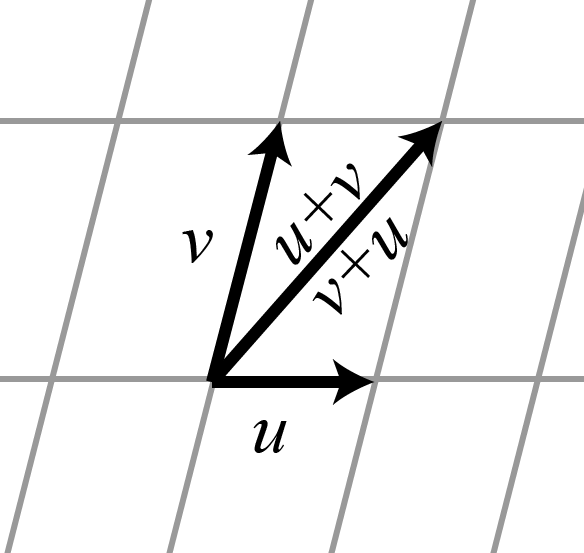
\includegraphics[scale=0.2]{images/21a.PNG}
\end{quotation}

\texttt{\tskcol{~~~~~~b) (s.)}}
\begin{quotation}
	\noindent
	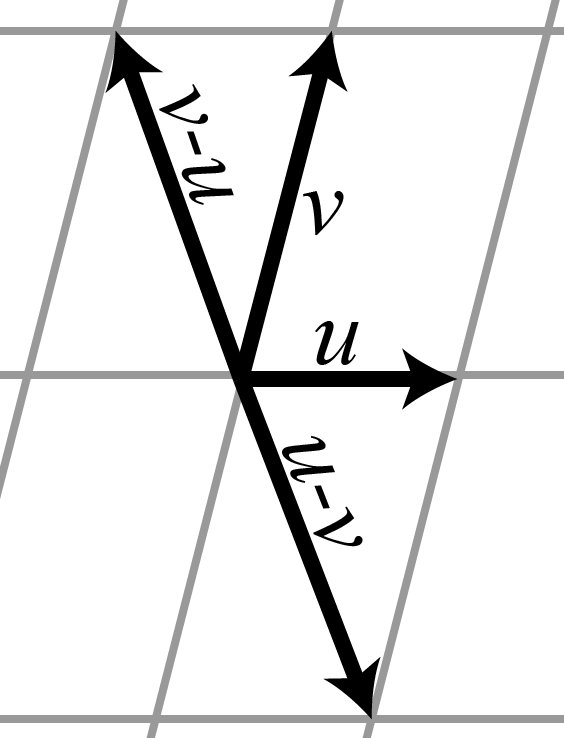
\includegraphics[scale=0.1]{images/21b.PNG}
\end{quotation}

\texttt{\tskcol{~~~~~~c) (s.)}}
\begin{quotation}
	\noindent
	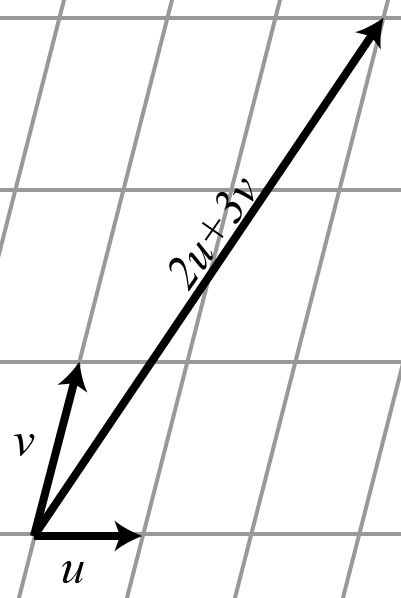
\includegraphics[scale=0.3]{images/21c.PNG}
\end{quotation}

\texttt{\tskcol{~~~~~~d) (s.)}}
\begin{quotation}
	\noindent
	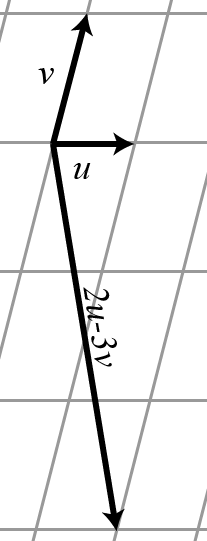
\includegraphics[scale=0.3]{images/21d.PNG}
\end{quotation}

\pagebreak
\texttt{\tskcol{2.2~~~~~ (s.)}}
\begin{quotation}
	\textbf{Svar:} Nollvektor
\end{quotation}

\texttt{\tskcol{2.3~~~~~ (s.)}}
\begin{quotation}
	\noindent
	Gausselimination:
	\begin{align*}
	&\left\{\begin{array}{rrr}
	 \hat{u}+& \hat{v}=&u \\
	2\hat{u}+&3\hat{v}=&u
	\end{array}\right.
	&\begin{array}{l}
	(a) \\
	(b)
	\end{array} \\ \Leftrightarrow
	&\left\{\begin{array}{rrr}
	\hat{u}+&\hat{v}=&u \\
	        &\hat{v}=&v-2u
	\end{array}\right.
	&\begin{array}{l}
	(a')=(a) \\
	(b')=(b)-2(a)
	\end{array} \\ \Leftrightarrow
	&\begin{cases}
	\hat{v}=v-2u \\
	\hat{u}=u-(v-2u)=3u-v
	\end{cases}
	\end{align*}
	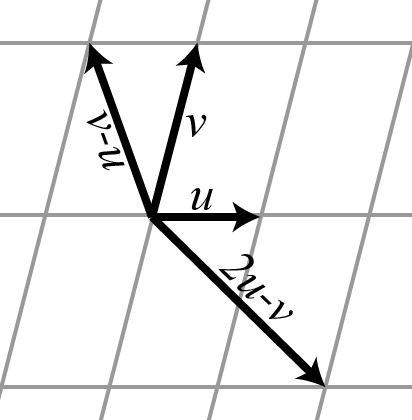
\includegraphics[scale=0.3]{images/23.PNG}
	\\ \\
	\textbf{Svar:} $\hat{v}=v-2u$, $\hat{u}=3u-v$
\end{quotation}

\texttt{\tskcol{2.4~~~~~ (s.)}}
\begin{quotation}
	\noindent
	\[\vek{OC}=\vek{OA}+\vek{AC}=\vek{OA}+\frac{1}{4}\vek{AB}\]
	\[\vek{OA}=\vek{OB}-\vek{AB} \Leftrightarrow
	\vek{AB}=\vek{OB}-\vek{OA}\]
	\[\vek{OC}=
	\vek{OA}+\frac{1}{4}\vek{AB}=
	\vek{OA}+\frac{1}{4}(\vek{OB}-\vek{OA})=
	\frac{3}{4}\vek{OA}-\frac{1}{4}\vek{OB} \text{~~~~V.S.V}\]
\end{quotation}

\texttt{\tskcol{2.5~~~~~ (s.)}}
\begin{quotation}
	\noindent
	\[\vek{OM}=\vek{OB}-\vek{MB}=\vek{OB}-\frac{1}{2}\vek{AB}\]
	\[\vek{OB}-\vek{AB}=\vek{OA}\Leftrightarrow
	\vek{AB}=\vek{OB}-\vek{OA}\]
	\[\vek{OM}=
	\vek{OB}-\frac{1}{2}\vek{AB}=
	\vek{OB}-\frac{1}{2}(\vek{OB}-\vek{OA})=
	\frac{1}{2}(\vek{OB}+\vek{OA}) \text{~~~~V.S.V}\]
\end{quotation}

\pagebreak
\texttt{\tskcol{2.6~~~~~ (s. 26-27)}}
\begin{quotation}
	\noindent
	Enligt uppgiften:
	\[\vek{AM}=\frac{2}{3}\vek{AA_1}\]
	Vilket ger:
	\[\vek{OM}=
	\vek{OA}+\vek{AM}=
	\vek{OA}+\frac{2}{3}\vek{AA_1}\]
	Mittpunktsformeln:
	\[\vek{AA_1}=\frac{1}{2}(\vek{AB}+\vek{AC})\]
	Vilket ger:
	\[\vek{OM}=
	\vek{OA}+\frac{2}{3}*\frac{1}{2}(\vek{AB}+\vek{AC})=
	\vek{OA}+\frac{1}{3}(\vek{AB}+\vek{AC})\]
	Enligt figuren:
	\[\vek{AB}=\vek{OB}-\vek{OA},~~
	\vek{AC}=\vek{OC}-\vek{OA}\]
	Vilket ger:
	\[\vek{OM}=
	\vek{OA}+\frac{1}{3}(\vek{OB}-\vek{OA}+\vek{OC}-\vek{OA})=
	\frac{1}{3}(\vek{OA}+\vek{OB}+\vek{OC}) \text{~~~~V.S.V}\]
\end{quotation}

\texttt{\tskcol{2.7~~~~~ (s.)}}
\begin{quotation}
	\noindent
	Enligt uppgiften:
	\[\vek{AM}=\frac{3}{4}\vek{AA_1}\]
	Vilket ger:
	\[\vek{OM}=
	\vek{OA}+\vek{AM}=
	\vek{OA}+\frac{3}{4}\vek{AA_1}\]
	Tyngdpunktsformeln:
	\[\vek{AA_1}=\frac{1}{3}(\vek{AB}+\vek{AC}+\vek{AD})\]
	Vilket ger:
	\[\vek{OM}=
	\vek{OA}+\frac{3}{4}*\frac{1}{3}(\vek{AB}+\vek{AC}+\vek{AD})=
	\vek{OA}+\frac{1}{4}(\vek{AB}+\vek{AC}+\vek{AD})\]
	Enligt figuren:
	\[\vek{AB}=\vek{OB}-\vek{OA},~~
	\vek{AC}=\vek{OC}-\vek{OA},~~
	\vek{AD}=\vek{OD}-\vek{OA}\]
	Vilket ger:
	\[\vek{OM}=
	\vek{OA}+\frac{1}{4}(\vek{OB}-\vek{OA}+\vek{OC}-\vek{OA}+\vek{OD}-\vek{OA})=
	\frac{1}{4}(\vek{OA}+\vek{OB}+\vek{OC}+\vek{OD}) \text{~~~~V.S.V}\]
\end{quotation}

\pagebreak
\texttt{\tskcol{2.8~~~~~ (s.)}}
\begin{quotation}
	\noindent
	Låt $O$ ligga i punkten $M$. tyngdpunktsformeln ger:
	\[\vek{OM}=\frac{1}{3}(\vek{OA}+\vek{OB}+\vek{OC})\]
	Eftersom $O=M$:
	\[\begin{cases}
	\vek{OM}=0 \\
	\vek{OA}=\vek{MA} \\
	\vek{OB}=\vek{MB} \\
	\vek{OC}=\vek{MC}
	\end{cases}\]
	Vilket ger:
	\[\frac{1}{3}(\vek{MA}+\vek{MB}+\vek{MC})=0 \Leftrightarrow
	\vek{MA}+\vek{MB}+\vek{MC}=3*0=0 \text{~~~~V.S.V}\]
\end{quotation}

\texttt{\tskcol{2.9~~~~~ (s.)}}
\begin{quotation}
	\noindent
	Låt $O$ vara en godtycklig punkt i rummet. Vilket ger:
	\[\begin{cases}
	\vek{A_1A_2}=\vek{OA_2}-\vek{OA_1} \\
	\vek{B_1B_2}=\vek{OB_2}-\vek{OB_1} \\
	\vek{C_1C_2}=\vek{OC_2}-\vek{OC_1}
	\end{cases}\]
	Tyngdpunktsformeln baklänges samt hur differens för vektorer funkar ger:
	\begin{align*}
	&\vek{A_1A_2}+\vek{B_1B_2}+\vek{C_1C_2}=
	\vek{OA_2}-\vek{OA_1}+\vek{OB_2}-\vek{OB_1}+\vek{OC_2}-\vek{OC_1}= \\ =
	&3*\frac{1}{3}(\vek{OA_2}+\vek{OB_2}+\vek{OC_2})-3*\frac{1}{3}(\vek{OA_1}+\vek{OB_1}+\vek{OC_1})= \\ =
	&3(\vek{OM_2}-\vek{OM_1})=
	3\vek{M_1M_2} \text{~~~~V.S.V}
	\end{align*}
\end{quotation}

\texttt{\tskcol{2.10~~~~ (s.)}}
\begin{quotation}
	\noindent
	Mittpunktsformeln ger:
	\[\begin{cases}
	\vek{OA_m}=\frac{1}{2}(\vek{OA}+\vek{OB}) \\
	\vek{OB_m}=\frac{1}{2}(\vek{OB}+\vek{OC}) \\
	\vek{OC_m}=\frac{1}{2}(\vek{OC}+\vek{OA})
	\end{cases}\]
	Vilket ger:
	\begin{align*}
	&VL=\vek{OA_m}+\vek{OB_m}+\vek{OC_m}=
	\frac{1}{2}(\vek{OA}+\vek{OB})+\frac{1}{2}(\vek{OB}+\vek{OC})+\frac{1}{2}(\vek{OC}+\vek{OA})= \\ =
	&\frac{1}{2}(2\vek{OA}+2\vek{OB}+2\vek{OC})=
	\vek{OA}+\vek{OB}+\vek{OC}=HL \text{~~~~V.S.V}
	\end{align*}
\end{quotation}

\pagebreak
\texttt{\tskcol{2.11~~~~ (s.)}}
\begin{quotation}
	\noindent
	Låt $ABCD$ vara en godtycklig tetraeder i rummet och $O$ vara en godtycklig punkt i rummet. 
	Om alla sammanbindningar skär tyngdpunkt vet vi även att alla skär varandra i tyngdpunkten.
	Antag att tyngdpunkten ligger i punkten $M$ och $\vek{OM}=\frac{1}{4}(\vek{OA}+\vek{OB}+\vek{OC}+\vek{OD})$.
	\\ \\
	Mittpunktsformeln ger:
	\[\begin{array}{lcr}
	p_1=\frac{1}{2}(\vek{OA}+\vek{OB}) & \text{~~~~motsatta punkt:~~~~} & q_1=\frac{1}{2}(\vek{OC}+\vek{OD}) \\
	p_2=\frac{1}{2}(\vek{OB}+\vek{OC}) & \text{~~~~motsatta punkt:~~~~} & q_2=\frac{1}{2}(\vek{OA}+\vek{OD}) \\
	p_3=\frac{1}{2}(\vek{OC}+\vek{OA}) & \text{~~~~motsatta punkt:~~~~} & q_3=\frac{1}{2}(\vek{OB}+\vek{OD})
	\end{array}\]
	En slumpmässig punkt på varje sammanbindning kan beskrivas som där $x,y,z$ ligger mellan 0 och 1:
	\[\begin{array}{l}
	s_1=p_1+x(q_1-p_1)=\frac{1}{2}(\vek{OA}+\vek{OB})+x\frac{1}{2}((\vek{OA}+\vek{OB})-(\vek{OC}+\vek{OD})) \\
	s_2=p_2+y(q_2-p_2)=\frac{1}{2}(\vek{OB}+\vek{OC})+y\frac{1}{2}((\vek{OB}+\vek{OC})-(\vek{OA}+\vek{OD})) \\
	s_2=p_3+z(q_3-p_3)=\frac{1}{2}(\vek{OC}+\vek{OA})+z\frac{1}{2}((\vek{OC}+\vek{OA})-(\vek{OB}+\vek{OD}))
	\end{array}\]
	Om vi sätter $x=y=z=\frac{1}{2}$ så kommer $s_1=s_2=s_3=\frac{1}{4}(\vek{OA}+\vek{OB}+\vek{OC}+\vek{OD})$ vilket är samma punkt som vi antog att tyngdpunkten $M$ skulle ligga i. Eftersom alla tre skär $M$ skär även alla tre varandra i $M$. ~~V.S.V
\end{quotation}

\texttt{\tskcol{2.12~~~~ (s.)}}
\begin{quotation}
	\noindent
	Låt $O$ vara en godtycklig punkt i rummet. 
	Om två stycken sträckor beskriver samma vektor måste de vara parallella enligt definitionen från vektorer. 
	Så om $\vek{A_1B_1}=\vek{D_1C_1}$ och $\vek{B_1C_1}=\vek{A_1D_1}$ är $A_1B_1C_1D_1$ en parallellogram.
	\\ \\
	mittpunktsformeln:
	\[\begin{array}{l}
	\vek{OA_1}=\frac{1}{2}(\vek{OA}+\vek{OB}) \\
	\vek{OB_1}=\frac{1}{2}(\vek{OB}+\vek{OC}) \\
	\vek{OC_1}=\frac{1}{2}(\vek{OC}+\vek{OD}) \\
	\vek{OD_1}=\frac{1}{2}(\vek{OD}+\vek{OA})
	\end{array}\]
	\[\begin{array}{l}
	\vek{A_1B_1}=\vek{OB_1}-\vek{OA_1}=\frac{1}{2}(\vek{OB}+\vek{OC}-(\vek{OA}+\vek{OB}))=\frac{1}{2}(\vek{OC}-\vek{OA}) \\
	\vek{D_1C_1}=\vek{OC_1}-\vek{OD_1}=\frac{1}{2}(\vek{OC}+\vek{OD}-(\vek{OD}+\vek{OA}))=\frac{1}{2}(\vek{OC}-\vek{OA}) \\
	\vek{B_1C_1}=\vek{OC_1}-\vek{OB_1}=\frac{1}{2}(\vek{OC}+\vek{OD}-(\vek{OB}+\vek{OC}))=\frac{1}{2}(\vek{OD}-\vek{OB}) \\
	\vek{A_1D_1}=\vek{OD_1}-\vek{OA_1}=\frac{1}{2}(\vek{OD}+\vek{OA}-(\vek{OA}+\vek{OB}))=\frac{1}{2}(\vek{OD}-\vek{OB})
	\end{array}\]
	$\vek{A_1B_1}=\vek{D_1C_1}$ och $\vek{B_1C_1}=\vek{A_1D_1}$ är alltså sant vilket innebär att $A_1B_1C_1D_1$ är en parallellogram. ~~V.S.V
\end{quotation}

\texttt{\tskcol{2.13~~a) (s.)}}
\begin{quotation}
	\noindent
	\[u_1=3e_1+2e_2\]
	\\
	\textbf{Svar:} $(3,2)$
\end{quotation}

\texttt{\tskcol{~~~~~~b) (s.)}}
\begin{quotation}
	\noindent
	\[u_2=2e_1+3e_2\]
	\\
	\textbf{Svar:} $(2,3)$
\end{quotation}

\texttt{\tskcol{~~~~~~c) (s.)}}
\begin{quotation}
	\noindent
	\[u_3=-2e_1+2e_2\]
	\\
	\textbf{Svar:} $(-2,2)$
\end{quotation}

\texttt{\tskcol{~~~~~~d) (s.)}}
\begin{quotation}
	\noindent
	\[u_4=-3e_1-2e_2\]
	\\
	\textbf{Svar:} $(-3,-2)$
\end{quotation}

\texttt{\tskcol{~~~~~~e) (s.)}}
\begin{quotation}
	\noindent
	\[u_5=2e_1-3e_2\]
	\\
	\textbf{Svar:} $(2,-3)$
\end{quotation}

\texttt{\tskcol{~~~~~~f) (s.)}}
\begin{quotation}
	\noindent
	\[e_1=1e_1+0e_2\]
	\\
	\textbf{Svar:} $(1,0)$
\end{quotation}

\texttt{\tskcol{~~~~~~g) (s.)}}
\begin{quotation}
	\noindent
	\[e_2=0e_1+1e_2\]
	\\
	\textbf{Svar:} $(0,1)$
\end{quotation}

\pagebreak
\texttt{\tskcol{2.14~~a) (s.)}}
\begin{quotation}
	\noindent
	$\hat{v}=v-2u$, $\hat{u}=3u-v$
	\begin{align*}
	&u=a\hat{u}+b\hat{v}=
	a(3u-v)+b(v-2u)=
	(3a-2b)u+(b-a)v \Leftrightarrow \\ \Leftrightarrow
	&\begin{cases}
	3a-2b=1 \\
	b-a=0
	\end{cases} \Leftrightarrow
	\begin{cases}
	a=1 \\ 
	b=1
	\end{cases} \Leftrightarrow
	u=1\hat{u}+1\hat{v}
	\end{align*}
	
	\begin{align*}
	&u=a\hat{u}+b\hat{v}=
	a(3u-v)+b(v-2u)=
	(3a-2b)u+(b-a)v \Leftrightarrow \\ \Leftrightarrow
	&\begin{cases}
	3a-2b=0 \\
	b-a=1
	\end{cases} \Leftrightarrow
	\begin{cases}
	a=2 \\ 
	b=3
	\end{cases} \Leftrightarrow
	u=2\hat{u}+3\hat{v}
	\end{align*}
	\\
	\textbf{Svar:} $u:~(1,1)$ och $v:~(2,3)$
\end{quotation}

\texttt{\tskcol{~~~~~~b) (s.)}}
\begin{quotation}
	\noindent
	\[\hat{u}=3u-v=3u-1v\]
	\[\hat{v}=v-2u=-2u+1v\]
	\\
	\textbf{Svar:} $\hat{u}:~(3,-1)$ och $\hat{v}:~(-2,1)$
\end{quotation}

\texttt{\tskcol{2.15~~~~ (s.)}}
\begin{quotation}
	\noindent
	\[\vek{OC}=\frac{3}{4}\vek{OA}+\frac{1}{4}\vek{OB}\]
	\\ 
	\textbf{Svar:} $\vek{OC}:~(3/4,1/4)$
\end{quotation}

\texttt{\tskcol{2.16~~~~ (s.)}}
\begin{quotation}
	\noindent
	För $\vek{TC}$ använd tyndpunktsformeln och låt $T$ vara den godtyckliga punkten i rummet.
	\[\vek{TT}=\frac{1}{3}(\vek{TA}+\vek{TB}+\vek{TC}) \Leftrightarrow
	0=\frac{1}{3}\vek{TA}+\frac{1}{3}\vek{TB}+\frac{1}{3}\vek{TC} \Leftrightarrow
	\vek{TC}=-\vek{TA}-\vek{TB}\]
	För $\vek{TM}$ använd mittpunktsformeln där $T$ är den godtyckliga punkten i rummet.
	\[\vek{TM}=\frac{1}{2}(\vek{TA}+\vek{TB})=\frac{1}{2}\vek{TA}+\frac{1}{2}\vek{TB}\]
	\\
	\textbf{Svar:} $\vek{TC}:~(-1,-1)$ och $\vek{TM}:~(1/2,1/2)$
\end{quotation}

\texttt{\tskcol{2.17~~a) (s.)}}
\begin{quotation}
	\noindent
	Vi ansätter lösningen:
	\[(4,1,-5)=x(2,1,-1)+y(1,1,1)\]
	Identifierar variablerna (gausselimination):
	\[\begin{cases}
	2x+y=4 \\
	x+y=1 \\
	-x+y=-5
	\end{cases} \Leftrightarrow
	\begin{cases}
	2x+y=4 \\
	y=-2 \\
	3y=-6
	\end{cases} \Leftrightarrow
	\begin{cases}
	x=3 \\
	y=-2
	\end{cases}\]
	\\ 
	\textbf{Svar:} $(4,1,-5)$ är en linjärkombination av $u_1$ och$u_2$
\end{quotation}

\texttt{\tskcol{~~~~~~b) (s.)}}
\begin{quotation}
	\noindent
	Vi ansätter lösningen:
	\[(4,3,2)=x(2,1,-1)+y(1,1,1)\]
	Identifierar variablerna (gausselimination):
	\[\begin{cases}
	2x+y=4 \\
	x+y=3 \\
	-x+y=2
	\end{cases} \Leftrightarrow
	\begin{cases}
	2x+y=4 \\
	y=2 \\
	3y=0
	\end{cases} \Leftrightarrow
	y=2\neq0 \Rightarrow \text{ Saknar lösning.}\]
	\\ 
	\textbf{Svar:} $(4,3,2)$ är inte en linjärkombination av $u_1$ och$u_2$
\end{quotation}

\texttt{\tskcol{~~~~~~c) (s.)}}
\begin{quotation}
	\noindent
	Vi ansätter lösningen:
	\[(-9,-7,-3)=x(2,1,-1)+y(1,1,1)\]
	Identifierar variablerna (gausselimination):
	\[\begin{cases}
	2x+y=-9 \\
	x+y=-7 \\
	-x+y=-3
	\end{cases} \Leftrightarrow
	\begin{cases}
	2x+y=-9 \\
	y=-5 \\
	3y=-15
	\end{cases} \Leftrightarrow
	\begin{cases}
	x=-7 \\
	y=-5
	\end{cases}\]
	\\ 
	\textbf{Svar:} $(-9,-7,-3)$ är en linjärkombination av $u_1$ och$u_2$
\end{quotation}

\texttt{\tskcol{2.18~~a) (s.)}}
\begin{quotation}
	\noindent
	För att två vektorer ska vara parallella ska det finnas ett $k$ så att:
	\[u=kv\]
	Ansätt därför en lösning och identifiera $k$ och $a$:
	\[(a,1+a)=k(2,-3) \Leftrightarrow
	\begin{cases}
	a=2k \\
	1+a=-3k
	\end{cases} \Leftrightarrow
	\begin{cases}
	a=-\frac{2}{5} \\
	k=-\frac{1}{5}
	\end{cases}\]
	\\
	\textbf{Svar:} $a=-\frac{2}{5}$
\end{quotation}

\texttt{\tskcol{~~~~~~b) (s.)}}
\begin{quotation}
	\noindent
	För att två vektorer ska vara parallella ska det finnas ett $k$ så att:
	\[u=kv\]
	Ansätt därför en lösning och identifiera $k$ och $a$:
	\[(a,-3)=k(2,1-a) \Leftrightarrow
	\begin{cases}
	a=2k \\
	-3=k(1-a)
	\end{cases}\]
	Substitutionsmetoden:
	\[-3=k(1-2k) \Leftrightarrow
	2k^2-k-3=0 \Leftrightarrow
	k^2-\frac{k}{2}-\frac{3}{2}=0\]
	\[k=\frac{1}{4}\pm\sqrt{\frac{1}{16}+\frac{24}{16}}=\frac{1}{4}\pm\frac{5}{4}\]
	\[\begin{cases}
	k_1=\frac{3}{2} \Leftrightarrow a_1=3 \\
	k_2=-1 \Leftrightarrow a_2=-2
	\end{cases}\]
	\\
	\textbf{Svar:} $a=3$ eller $a=-2$
\end{quotation}

\texttt{\tskcol{~~~~~~c) (s.)}}
\begin{quotation}
	\noindent
	För att två vektorer ska vara parallella ska det finnas ett $k$ så att:
	\[u=kv\]
	Ansätt därför en lösning och identifiera $k$ och $a$:
	\[(a,3)=k(2,1-a) \Leftrightarrow
	\begin{cases}
	a=2k \\
	3=k(1-a)
	\end{cases}\]
	Substitutionsmetoden:
	\[3=k(1-2k) \Leftrightarrow
	2k^2-k+3=0 \Leftrightarrow
	k^2-\frac{k}{2}+\frac{3}{2}=0\]
	\[k=\frac{1}{4}\pm\sqrt{\frac{1}{16}-\frac{24}{16}}=\frac{1}{4}\pm\sqrt{-\frac{23}{16}} \Rightarrow \text{ Saknar reell lösning}\]
	\\
	\textbf{Svar:} Saknar lösning
\end{quotation}

\texttt{\tskcol{~~~~~~d) (s.)}}
\begin{quotation}
	\noindent
	För att två vektorer ska vara parallella ska det finnas ett $k$ så att:
	\[u=kv\]
	Ansätt därför en lösning och identifiera $k$ och $a$:
	\[(a,1+a,3)=k(4,2,-6) \Leftrightarrow
	\begin{cases}
	a=4k \\
	1+a=2k \\
	3=-6k
	\end{cases} \Leftrightarrow
	\begin{cases}
	a=4k \\
	1=-2k \\
	3=-6k
	\end{cases} \Leftrightarrow
	\begin{cases}
	a=-2 \\
	k=-\frac{1}{2}
	\end{cases}\]
	\\
	\textbf{Svar:} $a=-2$
\end{quotation}

\texttt{\tskcol{2.19~~a) (s.)}}
\begin{quotation}
	\noindent
	För att vektorerna ska vara linjärt beroende ska de gå att beskriva med hjälp av varandra vilket innebär att det ska finnas ett $k$ så att:
	\[(2,4)=k(-4,-2)\]
	Identifiera variabeln:
	\[\begin{cases}
	2=-4k \\
	4=-2k
	\end{cases} \Leftrightarrow
	k=-\frac{1}{2}\neq-2 \Rightarrow \text{ saknar lösning}\]
	\\
	\textbf{Svar:} Vektorerna är inte linjärt beroende
\end{quotation}

\texttt{\tskcol{~~~~~~b) (s.)}}
\begin{quotation}
	\noindent
	För att vektorerna ska vara linjärt beroende ska de gå att beskriva med hjälp av varandra vilket innebär att det ska finnas ett $k$ så att:
	\[(6,-3)=k(-4,2)\]
	Identifiera variabeln:
	\[\begin{cases}
	6=-4k \\
	-3=2k
	\end{cases} \Leftrightarrow
	k=-\frac{3}{2}\]
	\\
	\textbf{Svar:} Vektorerna är linjärt beroende
\end{quotation}

\texttt{\tskcol{~~~~~~c) (s.)}}
\begin{quotation}
	\noindent
	För att vektorerna ska vara linjärt beroende ska de vara parallella och enligt definition är nollvektorn $(0,0)$ parallell med alla vektorer och därför är vektorerna linjärt beroende.
	\\ \\
	\textbf{Svar:} Vektorerna är linjärt beroende
\end{quotation}

\texttt{\tskcol{~~~~~~d) (s.)}}
\begin{quotation}
	\noindent
	För att vektorerna ska vara linjärt beroende ska de gå att beskriva med hjälp av varandra vilket innebär att det ska finnas ett $k_1$ och ett $k_2$ så att:
	\[(1,0)=k_1(0,1)+k_2(7,5)\]
	Identifiera variablerna:
	\[\begin{cases}
	1=7k_2 \\
	0=k_1+5k_2
	\end{cases} \Leftrightarrow
	\begin{cases}
	k_1=-\frac{5}{7} \\
	k_2=\frac{1}{7}
	\end{cases} \Rightarrow \text{ linjärt beroende}\]
	\\
	\textbf{Svar:} Vektorerna är linjärt beroende
\end{quotation}

\pagebreak
\texttt{\tskcol{~~~~~~e) (s.)}}
\begin{quotation}
	\noindent
	För att vektorerna ska vara linjärt beroende ska de gå att beskriva med hjälp av varandra vilket innebär att det ska finnas ett $k_1$ och ett $k_2$ så att:
	\[(5,9)=k_1(3,-2)+k_2(2,1)\]
	Identifiera variablerna:
	\[\begin{cases}
	5=3k_1+2k_2 \\
	9=-2k_1+k_2
	\end{cases} \Leftrightarrow
	\begin{cases}
	k_1=-\frac{13}{7} \\
	k_2=\frac{37}{7}
	\end{cases} \Rightarrow \text{ linjärt beroende}\]
	\\
	\textbf{Svar:} Vektorerna är linjärt beroende
\end{quotation}

\texttt{\tskcol{2.20~~a) (s.)}}
\begin{quotation}
	\noindent
	För att vektorerna ska vara linjärt beroende ska de gå att beskriva med hjälp av varandra vilket innebär att det ska finnas ett $k_1$ och ett $k_2$ så att:
	\[(1,1,1)=k_1(3,1,2)+k_2(0,2,1)\]
	Identifiera variablerna:
	\[\begin{cases}
	1=3k_1+0k_2 \\
	1=k_1+2k_2 \\
	1=2k_1+k_2
	\end{cases} \Leftrightarrow
	\begin{cases}
	k_1=\frac{1}{3} \\
	k_2=\frac{1}{3}
	\end{cases} \Rightarrow \text{ linjärt beroende}\]
	\\
	\textbf{Svar:} Vektorerna är linjärt beroende
\end{quotation}

\texttt{\tskcol{~~~~~~b) (s.)}}
\begin{quotation}
	\noindent
	För att vektorerna ska vara linjärt beroende ska de gå att beskriva med hjälp av varandra vilket innebär att det ska finnas ett $k_1$ och ett $k_2$ så att:
	\[(0,1,1)=k_1(1,0,1)+k_2(1,1,0)\]
	Identifiera variablerna:
	\[\begin{cases}
	0=k_1+k_2 \\
	1=0k_1+k_2 \\
	1=k_1+0k_2
	\end{cases} \Leftrightarrow
	\begin{cases}
	k_1=1 \\
	k_2=1\neq-1
	\end{cases} \Rightarrow \text{ linjärt oberoende}\]
	\\
	\textbf{Svar:} Vektorerna är inte linjärt beroende
\end{quotation}

\texttt{\tskcol{~~~~~~c) (s.)}}
\begin{quotation}
	\noindent
	För att vektorerna ska vara linjärt beroende ska de gå att beskriva med hjälp av varandra vilket innebär att det ska finnas ett $k$ så att:
	\[(1,1,1)=k(3,1,2)\]
	Identifiera variabeln:
	\[\begin{cases}
	1=3k \\
	1=k \\
	1=2k
	\end{cases} \Leftrightarrow
	k=\frac{1}{3}\neq1\neq\frac{1}{2} \Rightarrow \text{ linjärt oberoende}\]
	\\
	\textbf{Svar:} Vektorerna är inte linjärt beroende
\end{quotation}

\texttt{\tskcol{~~~~~~d) (s.)}}
\begin{quotation}
	\noindent
	För att vektorerna ska vara linjärt beroende ska de gå att beskriva med hjälp av varandra vilket innebär att det ska finnas ett $k$ så att:
	\[(1,0,2)=k(-2,0,-4)\]
	Identifiera variabeln:
	\[\begin{cases}
	1=-2k \\
	0=0k \\
	2=-4k
	\end{cases} \Leftrightarrow
	k=-\frac{1}{2} \Rightarrow \text{ linjärt beroende}\]
	\\
	\textbf{Svar:} Vektorerna är linjärt beroende
\end{quotation}

\texttt{\tskcol{~~~~~~e) (s.)}}
\begin{quotation}
	\noindent
	Eftersom $(1,0,2)$ och $(-2,0,-4)$ är linjärt beroende (se \texttt{\tskcol{d)}}) är även $(2,0,3)$, $(1,0,2)$ och $(-2,0,-4)$ det.
	\\ \\
	\textbf{Svar:} Vektorerna är linjärt beroende
\end{quotation}

\texttt{\tskcol{~~~~~~f) (s.)}}
\begin{quotation}
	För att vektorerna ska vara linjärt beroende ska de gå att beskriva med hjälp av varandra vilket innebär att det ska finnas ett $k_1$ och ett $k_2$ så att:
	\[(1,0,2)=k_1(3,0,4)+k_2(5,0,6)\]
	Identifiera variablerna (gausselimination):
	\[\begin{cases}
	1=3k_1+5k_2 \\
	0=0k_1+0k_2 \\
	2=4k_1+6k_2
	\end{cases} \Leftrightarrow
	\begin{cases}
	k_1=2 \\
	k_2=-1
	\end{cases}\Rightarrow \text{ linjärt beroende}\]
	\\
	\textbf{Svar:} Vektorerna är linjärt beroende
\end{quotation}

\texttt{\tskcol{~~~~~~g) (s.)}}
\begin{quotation}
	\noindent
	För att vektorerna ska vara linjärt beroende ska de gå att beskriva med hjälp av varandra vilket innebär att det ska finnas ett $k_1$, ett $k_2$ och ett $k_3$ så att:
	\[(1,1,0)=k_1(1,0,1)+k_2(0,1,1)+k_3(3,3,3)\]
	Identifiera variablerna (gausselimination):
	\[\begin{cases}
	1=k_1+0k_2+3k_3 \\
	1=0k_1+k_2+3k_3 \\
	0=k_1+k_2+3k_3
	\end{cases} \Leftrightarrow
	\begin{cases}
	k_1=-1 \\
	k_2=-1 \\
	k_3=\frac{2}{3}
	\end{cases}\Rightarrow \text{ linjärt beroende}\]
	\\
	\textbf{Svar:} Vektorerna är linjärt beroende
\end{quotation}

\texttt{\tskcol{2.21~~~~ (s.)}}
\begin{quotation}
	\noindent
	För att vektorerna ska vara linjärt beroende ska de gå att beskriva med hjälp av varandra (de ska vara parallella) vilket innebär att det ska finnas ett $k$ och $a$ så att:
	\[(a,-2)=k(1,a-1)\]
	Identifiera variabeln:
	\[\begin{cases}
	a=k \\
	-2=k(a-1)
	\end{cases}\]
	Substitutionsmetoden:
	\[-2=k(k-1) \Leftrightarrow
	k^2-k+2=0\]
	\[k=\frac{1}{2}\pm\sqrt{\frac{1}{4}-\frac{8}{4}}=\frac{1}{2}\pm\sqrt{-\frac{7}{4}} \Rightarrow \text{ saknar reell lösning}\]
	\\
	\textbf{Svar:} Nej, det finns inget $a$ så att vektorerna är linjärt beroende
\end{quotation}

\texttt{\tskcol{2.22~~a) (s.)}}
\begin{quotation}
	\noindent
	\[u=5e_1+3e_2\]
	\\
	\textbf{Svar:} $(5,3)$
\end{quotation}

\texttt{\tskcol{~~~~~~b) (s.)}}
\begin{quotation}
	\noindent
	Ja, eftersom de inte är parallella.
	\\ \\
	\textbf{Svar:} Ja
\end{quotation}

\texttt{\tskcol{~~~~~~c) (s.)}}
\begin{quotation}
	\noindent
	\[2\hat{e}_1+\hat{e}_2=u\]
	\\ \\
	\textbf{Svar:} $(2,1)$
\end{quotation}

\texttt{\tskcol{~~~~~~d) (s.)}}
\begin{quotation}
	\noindent
	\[\hat{e}_1=e_1+2e_2 \Rightarrow (1,2)\]
	\[\hat{e}_2=3e_1-e_2 \Rightarrow (3,-1)\]
	\\
	\textbf{Svar:} $\hat{e}_1:~(1,2)$ och $\hat{e}_2:~(3,-1)$
\end{quotation}

\pagebreak
\texttt{\tskcol{~~~~~~e) (s.)}}
\begin{quotation}
	\noindent
	\begin{align*}
	&x_1e_1+x_2e_2=v=
	\hat{x}_1\hat{e}_1+\hat{x}_2\hat{e}_2=
	\hat{x}_1(e_1+2e_2)+\hat{x}_2(3e_1-e_2)= \\ =
	&(\hat{x}_1+3\hat{x}_2)e_1+(2\hat{x}_1-\hat{x}_2)e_2 \Rightarrow (x_1,x_2)=(\hat{x}_1+3\hat{x}_2,2\hat{x}_1-\hat{x}_2)
	\end{align*}
\end{quotation}

\texttt{\tskcol{2.23~~~~ (s.)}}
\begin{quotation}
	\noindent
	$\hat{e}_1$ och $\hat{e}_2$ kan användas som bas om de inte är parallella så genom att anta att de är parallella kan vi bestämma om de kan användas som bas eller inte. De är parallella om det finns ett $k$ så att:
	\[\hat{e}_1=k\hat{e}_2\] 
	\[\hat{e}_1=k\hat{e}_2 \Leftrightarrow
	-e_1+2e_2=k(3e_1+4e_2) \Leftrightarrow
	\begin{cases}
	-1=3k \\
	2=4k
	\end{cases} \Leftrightarrow
	k=-\frac{1}{3}\neq\frac{1}{2}\]
	Linjerna är inte parallella och därför kan de vara en bas i planet.
	\begin{align*}
	&\begin{cases}
	\hat{e}_1=-e_1+2e_2 \\
	\hat{e}_2=3e_1+4e_2
	\end{cases} \Leftrightarrow
	\begin{cases}
	e_1=-\hat{e}_1+2e_2 \\
	e_2=\frac{1}{4}\hat{e}_2-\frac{3}{4}e_1
	\end{cases}\Leftrightarrow \\ \Leftrightarrow
	&\begin{cases}
	e_1=-\hat{e}_1+2(\frac{1}{4}\hat{e}_2-\frac{3}{4}e_1) \\
	e_2=\frac{1}{4}\hat{e}_2-\frac{3}{4}(-\hat{e}_1+2e_2)
	\end{cases}\Leftrightarrow
	\begin{cases}
	e_1=-\frac{2}{5}\hat{e}_1+\frac{1}{5}\hat{e}_2 \\
	e_2=\frac{3}{10}\hat{e}_1+\frac{1}{10}\hat{e}_2
	\end{cases}
	\end{align*}
	Sätt sedan in i uttrycket för vektorn.
	\begin{align*}
	&u=4e_1-5e_2=
	4(-\frac{2}{5}\hat{e}_1+\frac{1}{5}\hat{e}_2)-5(\frac{3}{10}\hat{e}_1+\frac{1}{10}\hat{e}_2)= \\ =
	&-\frac{8}{5}\hat{e}_1-\frac{15}{10}\hat{e}_1+\frac{4}{5}\hat{e}_2-\frac{5}{10}\hat{e}_2=
	-\frac{31}{10}\hat{e}_1+\frac{3}{10}\hat{e}_2
	\end{align*}
	\\
	\textbf{Svar:} $(-3.1,0.3)$
\end{quotation}

\pagebreak
\texttt{\tskcol{2.24~~a) (s.)}}
\begin{quotation}
	\noindent
	För att visa att $e^{'}_1$, $e^{'}_2$ och $e^{'}_3$ är en bas i rummet behöver vi först visa att  $e^{'}_1$ och $e^{'}_2$ är linjärt oberoende i planet och sedan visa att $e^{'}_3$ är linjärt oberoende i rummet.
	\\ \\
	Om det inte finns $k$ så att:
	\[e^{'}_1=ke^{'}_2\]
	är $e^{'}_1$ och $e^{'}_2$ linjärt oberoende i planet.
	\begin{align*}
	&e^{'}_1=ke^{'}_2 \Leftrightarrow
	e^1+0e^2+0e^3=k(2e^1+e^2+0e^3) \Leftrightarrow \\ \Leftrightarrow
	&\begin{cases}
	1=2k \\
	0=k \\
	0=0
	\end{cases} \Leftrightarrow
	k=\frac{1}{2}\neq0 \Leftrightarrow
	\text{ linjärt oberoende}
	\end{align*}
	Om det inte finns $k_1$ och $k_2$ så att:
	\[e^{'}_3=k_1e^{'}_1+k_2e^{'}_2\]
	är $e^{'}_1$, $e^{'}_2$ och $e^{'}_3$ linjärt oberoende i rummet.
	\begin{align*}
	&e^{'}_3=k_1e^{'}_1+k_2e^{'}_2 \Leftrightarrow \\ \Leftrightarrow
	&3e^1+2e^2+e^3=k_1(e^1+0e^2+0e^3)+k_2(2e^1+e^2+0e^3) \Leftrightarrow \\ \Leftrightarrow
	&\begin{cases}
	3=k_1+2k_2 \\
	2=k_2 \\
	1\neq0
	\end{cases} \Leftrightarrow
	1\neq0 \Leftrightarrow
	\text{ linjärt oberoende}
	\end{align*}
	$e^{'}_1$, $e^{'}_2$ och $e^{'}_3$ är en bas i rummet.
\end{quotation}

\texttt{\tskcol{~~~~~~b) (s.)}}
\begin{quotation}
	\noindent
	\[x^{'}_1e^{'}_1+x^{'}_2e^{'}_2+x^{'}_3e^{'}_3=x_1e_1+x_2e_2+x_3e_3\]
	\begin{align*}
	VL=&x^{'}_1(e_1)+x^{'}_2(2e_1+e_2)+x^{'}_3(3e_1+2e_2+e_3)= \\ =
	&(x^{'}_1+2x^{'}_2+3x^{'}_3)e_1+(x^{'}_2+2x^{'}_3)e_2+x^{'}_3e_3
	\end{align*}
	identifiera variablerna:
	\[\begin{cases}
	x_1=x^{'}_1+2x^{'}_2+3x^{'}_3 \\
	x_2=x^{'}_2+2x^{'}_3 \\
	x_3=x^{'}_3
	\end{cases}\]
\end{quotation}

\pagebreak
\texttt{\tskcol{~~~~~~c) (s.)}}
\begin{quotation}
	\noindent
	\[u=
	2e_1+7e_3 \Leftrightarrow
	\begin{cases}
	2=x^{'}_1+2x^{'}_2+3x^{'}_3 \\
	0=x^{'}_2+2x^{'}_3 \\
	7=x^{'}_3
	\end{cases} \Leftrightarrow
	\begin{cases}
	x^{'}_3=7 \\
	x^{'}_2=-14 \\
	x^{'}_1=9
	\end{cases}\]
	\\
	\textbf{Svar:} $(x^{'}_1,x^{'}_2,x^{'}_3)=(9,-14,7)$
\end{quotation}

\texttt{\tskcol{2.25~~~~ (s.)}}
\begin{quotation}
	\noindent
	Visa att $\hat{e}_1$, $\hat{e}_2$ och $\hat{e}_3$ är linjärt oberoende.
	\begin{align*}
	&\lambda_1\hat{e}_1+\lambda_2\hat{e}_2+\lambda_3\hat{e}_3=0 \Leftrightarrow \\ \Leftrightarrow
	&\lambda_1(e_1+e_2)+\lambda_2(e_1+e_2-e_3)+\lambda_3(e_2-e_3)=0 \Leftrightarrow \\ \Leftrightarrow
	&(\lambda_1+\lambda_2)e_1+(\lambda_1+\lambda_2+\lambda_3)e_2+(-\lambda_2-\lambda_3)e_3=0 \Leftrightarrow \\ \Leftrightarrow
	&\begin{cases}
	0=\lambda_1+\lambda_2 \\
	0=\lambda_1+\lambda_2+\lambda_3 \\
	0=-\lambda_2-\lambda_3 \\
	\end{cases}
	\end{align*}
	Enda lösningen är $\lambda_1=\lambda_2=\lambda_3=0$ vilket innebär att de är linjärt oberoende och där med en möjlig bas i rummet.
	\[u=2e_1+3e_2-2e_3=\hat{x}_1\hat{e}_1+\hat{x}_2\hat{e}_2+\hat{x}_3\hat{e}_3\]
	\begin{align*}
	HL=&\hat{x}_1(e_1+e_2)+\hat{x}_2(e_1+e_2-e_3)+\hat{x}_3(e_2-e_3)= \\ =
	&(\hat{x}_1+\hat{x}_2)e^1+(\hat{x}_1+\hat{x}_2+\hat{x}_3)e^2+(-\hat{x}_2-\hat{x}_3)e^3
	\end{align*}
	Identifiera variablerna (gausselimination):
	\[\begin{cases}
	2=\hat{x}_1+\hat{x}_2 \\
	3=\hat{x}_1+\hat{x}_2+\hat{x}_3 \\
	-2=-\hat{x}_2-\hat{x}_3
	\end{cases} \Leftrightarrow
	\begin{cases}
	2=\hat{x}_1+\hat{x}_2 \\
	1=\hat{x}_3 \\
	-2=-\hat{x}_2-\hat{x}_3
	\end{cases} \Leftrightarrow
	\begin{cases}
	\hat{x}_3=1 \\
	\hat{x}_2=1 \\
	\hat{x}_1=1
	\end{cases}
	\]
	\\
	\textbf{Svar:} $(1,1,1)$
\end{quotation}

\texttt{\tskcol{2.26~~~~ (s.)}}
\begin{quotation}
	\noindent
	\\ \\
	\textbf{Svar:}
\end{quotation}

\texttt{\tskcol{2.27~~~~ (s.)}}
\begin{quotation}
	\noindent
	\\ \\
	\textbf{Svar:}
\end{quotation}

\texttt{\tskcol{2.28~~a) (s.)}}
\begin{quotation}
	\noindent
	\\ \\
	\textbf{Svar:}
\end{quotation}

\texttt{\tskcol{~~~~~~b) (s.)}}
\begin{quotation}
	\noindent
	\\ \\
	\textbf{Svar:}
\end{quotation}

\texttt{\tskcol{2.29~~~~ (s.)}}
\begin{quotation}
	\noindent
	\\ \\
	\textbf{Svar:}
\end{quotation}

\texttt{\tskcol{2.30~~~~ (s.)}}
\begin{quotation}
	\noindent
	\\ \\
	\textbf{Svar:}
\end{quotation}
\end{document}